
\documentclass[fleqn]{exam}
\usepackage{amsmath}
\usepackage{graphicx}
\usepackage{booktabs}
\usepackage{float}
\usepackage{caption}
\usepackage{polynom}
\usepackage{mdwlist}
\usepackage{cancel}
\usepackage{fullpage}

\usepackage{parskip}
\usepackage{paralist}

\usepackage{unitsdef} 
\newunit{\inch}{in}
\newunit{\mile}{mile}
\newunit{\mph}{mph}
\newunit{\foot}{ft}
\newunit{\knot}{knot}
\newunit{\gallon}{gallon}

\setcounter{tocdepth}{2}

\everymath{\displaystyle}


% \begin{figure}[H]
%   \centering
%   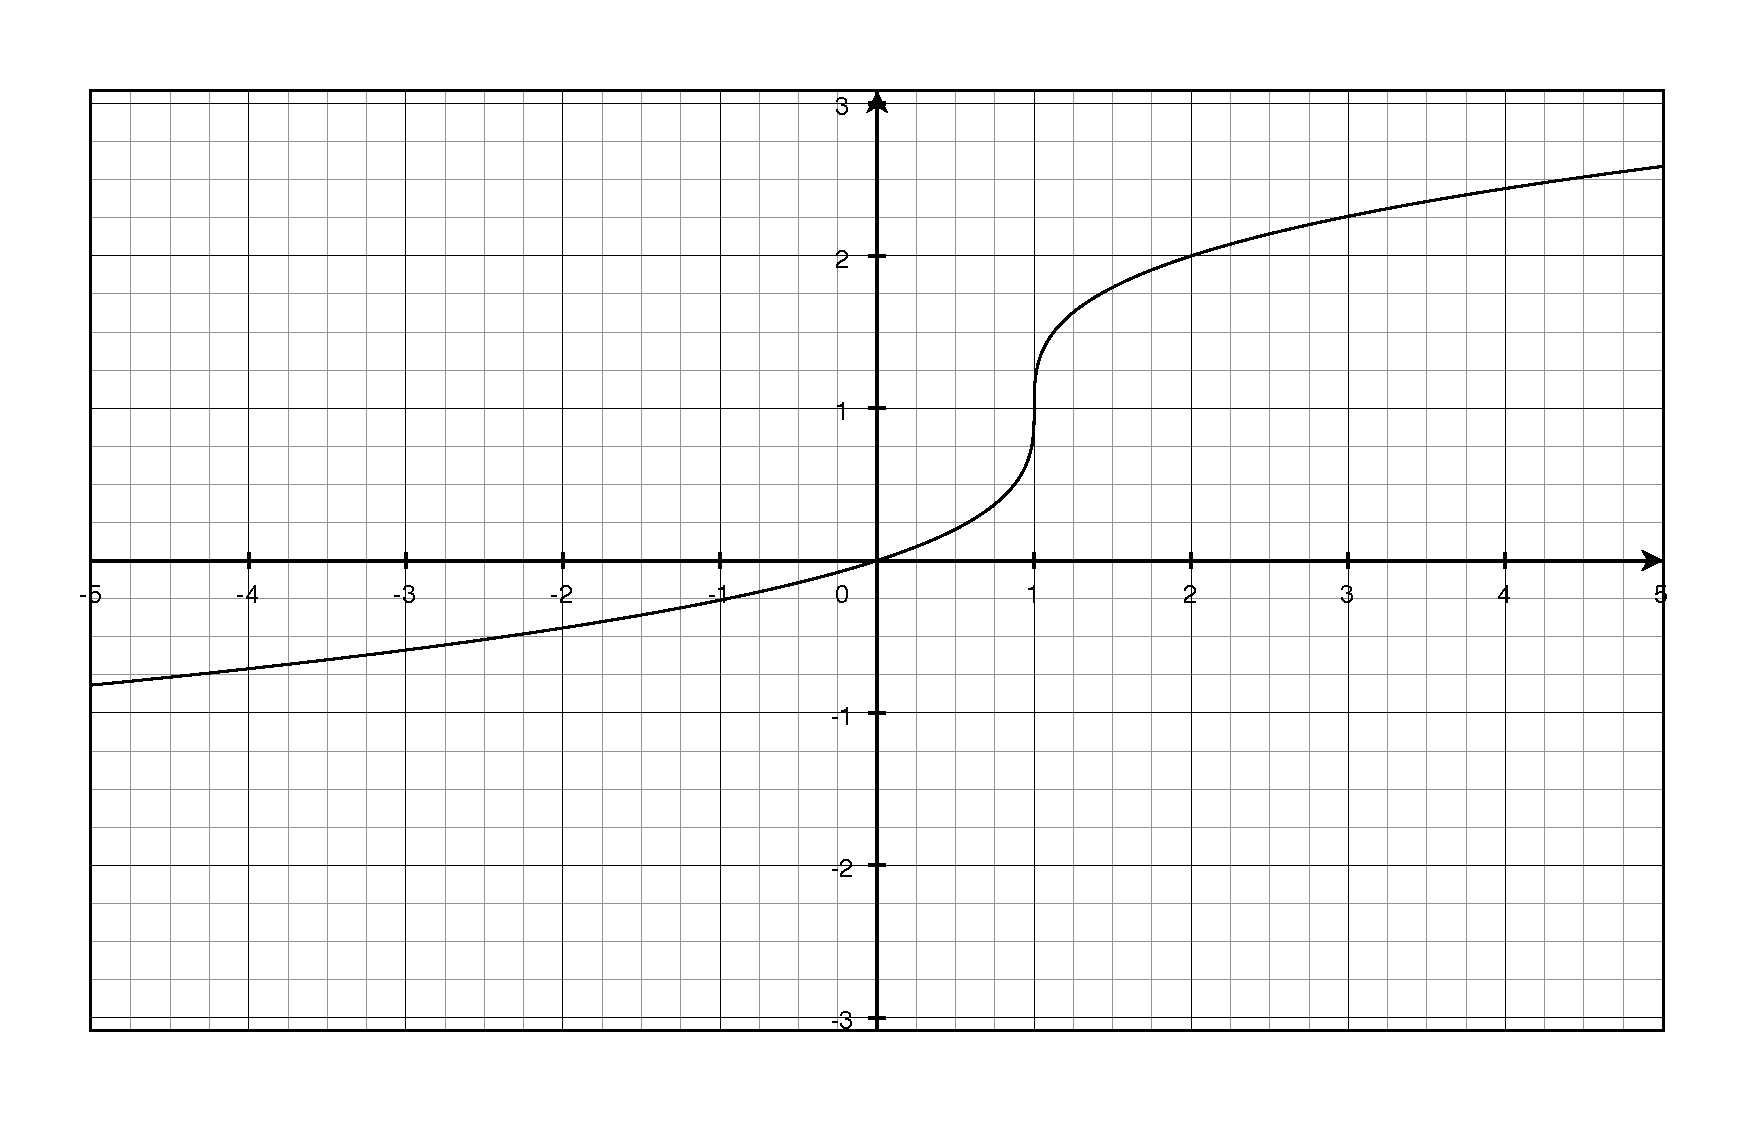
\includegraphics[scale=.3]{question7.eps}
%   \caption*{Question 7}
% \end{figure}

% \begin{tabular}{cc}
% \toprule
% period & amplitude \\
% \midrule
%   $\pi$ & $2$ \\
% \bottomrule
% \end{tabular}

\printanswers

%% \ifprintanswers
%% \usepackage{2in1, lscape}
%% \fi

\title{Math 263A \\ Chapter Three Study Guide \\ Derivatives}
\date{October 11, 2012}

\author{}

\begin{document}

\maketitle  

\section{Derivative Definition}

The derivative of a function is a new function which provides the slope, or instantaneous rate of change, of the
original function at any point.

There are several equivalent definitions of the derivative:
\begin{align*}
  f'(x) &= \lim_{h \to 0} \frac{f(x + h) - f(x)}{h} \\
  f'(c) &= \lim_{x \to c} \frac{f(x) - f(c)}{x - c} \\
\end{align*}
You should know both of these definitions and be able to use them to find derivatives.  

\section{Notation}
There are three notations for the derivative:
\begin{itemize*}
\item $D_x f(x)$
\item $f'(x)$
\item $\frac{dy}{dx}$
\end{itemize*}

\section{Rules for Finding Derivatives}
Finding derivatives using the definition is fairly tedious.  Fortunately, there are some rules you can memorize which
allow you to quickly find the derivatives for many functions.

\subsection{Constant Multiple}
You can move a constant around without changing the result:
\[
  D_x k f(x) = k f'(x) 
\]

\subsection{Power}
The derivative of $x$ raised to a power is:
\[
  D_x x^n = n x^{n - 1}
\]
The power can be any rational number.

\subsection{Constant Function}
A special case of the power rule is when the exponent is 0 and the function is just a constant.  In this case, the derivative is also zero, which makes
sense because the slope of a constant function is zero

\subsection{Sum/Difference}
The derivative of the sum of two functions is the same as the sum of the two derivatives: 
\[
  D_x [ f(x) \pm g(x) ] = f'(x) \pm g'(x)
\]

\subsection{Product}
The rule for the product of two functions is:
\[
  D_x [ f(x) g(x) ] = g(x) f'(x) + f(x) g'(x)
\]

\subsection{Quotient}
The rule for the quotient of two functions is:
\[
  D_x \frac{f(x)}{g(x)} = \frac{g(x) f'(x) - f(x) g'(x)}{g^2(x)}
\]

\subsection{Composition of Functions/Chain Rule}
The rule for the composition of two functions is:
\[
  D_x [ (f \circ g) (x) ] = f'(g(x)) \cdot g'(x)
\]

\section{Derivatives of Trigonometric Functions}
The derivatives of some common trigonometric functions are:
\begin{align*}
  D_x \sin x &= \cos x \\
  D_x \cos x &= - \sin x \\
  D_x \tan x &= \sec^2 x \\
\end{align*}

You can figure all the other ones out using the derivative rules.  All you really need to memorize are the sine and
cosine derivatives.

\section{Higher Order Derivatives}
You don't have to stop after taking one derivative.  Since a derivative is a function, you can take the derivative of a
derivative, the derivative of the derivative of a derivative, etc.  

The notation choices for second derivative are:
\[
  D_x (D_x f(x)) = D_x^2 f(x) = f''(x) = \frac{d^2}{dx^2} f(x) \\
\]

An example of second derivative is:
\begin{itemize*}
  \item velocity is the rate of change of the position, or the first derivative of the position
  \item acceleration is the rate of change of the velocity, or the second derivative of the position
\end{itemize*}

\section{Implicit Differentiation}

Sometimes when you have an equation with two variables, it's difficult to solve for one of the variables in terms of the
other.  In this case, you can use {\em implicit differentiation} to find the derivative.  

The general approach is:
\begin{enumerate*}
  \item Take the derivative of both sides.  If you're trying to find $\frac{dy}{dx}$, $y$ is a function of $x$, so you
    will need to use the chain rule.
  \item Solve for $\frac{dy}{dx}$.
\end{enumerate*}

Usually the final result will be in terms of both $x$ and $y$.  This means that if you are looking for the value at a
particular point, you'll need to know both the $x$ and $y$ values for the point you're interested in.

\section{Related Rates}
\label{related-rates}

If you are trying to find the rate something changes with respect to time and have:
\begin{itemize*}
  \item an expression for the quantity you're interested in, in terms of some other quantity
  \item the rate the other quantity changes with respect to time
\end{itemize*}
then you can find the rate you're interested in:
\begin{itemize*}
  \item differentiate both sides of the equation you have with respect to time.  Remember to apply the chain rule, where
    appropriate.
  \item Substitute the rate and values you have to get the answer.
\end{itemize*}

\subsection{Moving Objects}

If you see a problem with two objects moving at right angles to each other and are asked to find the rate at which the
distance between them is changing, you have a {\em Moving Objects Related Rate} problem.  The objects might be cars,
boats, planes, walking people, dogs, etc.

Other problems which use exactly the same math but seem different at first are:
\begin{itemize}
\item A kite traveling horizontally at a fixed horizontal speed and height.  In this case, $\frac{dy}{dt} = 0$ (no
  change in height), and you need to find either $\frac{dr}{dx}$ (rate of change of string length) or $\frac{dx}{dt}$
  (horizontal speed).
\item An airplane traveling overhead at a fixed altitude.  This is the same as the kite problem with an airplane instead
  of a kite.
\end{itemize}

The key parts of this type of problem are:
\begin{itemize*}
\item Often the objects start moving at different times.
\item Often the objects are moving at different speeds.  Sometimes one of the objects is stationary.
\item If both objects are moving, one object is moving along the x axis and the other object is moving along the y axis.
\end{itemize*}

The final equation for this type of problem generally looks like this:
\[
  \frac{dr}{dt} = \frac{y}{r} \cdot \frac{dy}{dt} + \frac{x}{r} \cdot \frac{dx}{dt}
\]

This equation makes sense:
\begin{itemize}
  \item If $\frac{y}{r} \approx 1$, then $\frac{x}{r} \approx 0$ and most of the change in the total distance comes from
    the y direction.  For example if one car is in Portland heading towards Los Angeles and the other is in Seattle
    heading towards Yakima, most of the change in distance between the two cars comes from the Portland car.

  \item if $\frac{dy}{dt}$ is a lot bigger than $\frac{dx}{dt}$, then the y speed affects the total more than the x
    speed.  For example if a car and a bicycle start out together in Seattle, with the car going south and the bike
    going east, most of the change in the distance between them comes from the car.
 
\end{itemize}

The steps for solving this type of problem are:
\begin{itemize*}
  \item Have one object move along the x axis and the other object move along the y axis
  \item Find expressions for x and y in terms of time.  Be careful about the direction (positive or negative) each
    object is moving in
  \item Let $r$ be the distance between the two objects
  \item Use the Pythagorean theorem to find an expression for $r^2$ in terms of $x$ and $y$.  $r^2$ is usually better
    than $r$ because it makes the differentiation easier.
  \item Use implicit differentiation to get the expression shown above.
  \item Substitute in the rates and distances you have and solve for the missing rate.
\end{itemize*}

\subsection{Volume}

You have some oddly shaped object which is gradually being filled with water.  You know the rate the volume is changing
(the rate the water is going in) and want to know the rate the height is changing.  The steps are:

\begin{itemize*}
\item write down all the equations you can think of for height, width, radius, volume, etc.
\item find an expression for the volume in terms of just one height/width/radius variable by solving one of the other
  equations for one of these and substituting it in the volume equation
\item use implicit differentiation to get $\frac{dV}{dt}$ in terms of $\frac{dh}{dt}$, etc.
\item plug in the values you know and solve for whatever you are missing
\end{itemize*}

\section{Differentials and Approximations}
{\em Differentials} are used to approximate how much $y$ changes when $x$ changes by a small amount.  Differentials are
defined by thinking of $\frac{dy}{dx}$ as a fraction and solving for $dy$:
\begin{align*}
  \frac{dy}{dx} &= f'(x) \\
  dy &= f'(x) dx \\
\end{align*}

To use differentials to approximate:
\begin{itemize*}
\item find the derivative of the function
\item multiply the derivative by the change in $x$ to find approximately how much $y$ changes.
\end{itemize*}

%% For example, to find $\sqrt{402}$, we know that it is approximately $\sqrt{400}$ plus a bit more:
%% \begin{align*}
%%   f(x) &= x^{1/2} \\
%%   dy &= \frac{1}{2 \sqrt{x}} \cdot \, dx \\
%%      &= \frac{1}{2 \sqrt{400}} \cdot 2 \\
%%      &= \frac{1}{20} \\
%%      &= 0.05 \\
%% \\
%%   \sqrt{402} \approx 20.05 \\
%% \end{align*}


\end{document}
